\section{Problem statement and model}
\label{sec:Chapter_III}
\subsection{Problem statement}

An instance is a set of jobs, robotic arms, and vehicles on a shop-floor graph (Table~\ref{tab:notation}).
Each job is a fixed operation chain; each operation has an option set of arms with machine-dependent processing times.
Arms occupy fixed nodes; the fleet moves jobs between them.
Four decisions are taken at once:
(i)~assign each operation to an optional arm;
(ii)~sequence each arm;
(iii)~assign and sequence the induced transport tasks on vehicles;
(iv)~plan a conflict-free path for every move, waits allowed.
The objective is to minimize $C_{\max}$.

\begin{table}[t]
\caption{Notation.}
\label{tab:notation}
\footnotesize
\renewcommand{\arraystretch}{0.95}
\begin{tabular}{@{}ll@{}}
\toprule
Symbol & Meaning \\
\midrule
$J=\{1,\dots,n\}$, $O_{ji}$ & jobs; $i$-th operation of job $j$, $i\le n_j$ \\
$M=\{1,\dots,N_M\}$, $\Omega_{ji}\subseteq M$ & robotic arms; option set of $O_{ji}$ \\
$t^P_{jim}$ & processing time of $O_{ji}$ on arm $m\in\Omega_{ji}$ \\
$K=\{1,\dots,N_A\}$ & homogeneous unit-load vehicles \\
$G=(V,E)$, $\tau_e$ & shop-floor graph; traversal time of corridor $e$ \\
$v_0$, $\mathrm{loc}(m)$ & load/unload point; node of arm $m$ \\
$t^{*}(a,b)$ & shortest-path time $a\to b$ in $G$, ignoring contention \\
$\delta_{\mathrm{ret}}\in\{0,1\}$ & finished job returns to $v_0$ (baseline $1$) \\
$S_{ji}$, $C_{ji}$, $A_{ji}$, $C_{\max}$ & start, completion, arrival; makespan \\
\bottomrule
\end{tabular}
\end{table}

\subsection{Modelling assumptions}
\label{sec:assumptions}

\begin{enumerate}[label=\textbf{A\arabic*.},leftmargin=*,topsep=2pt,itemsep=1pt]
\item \textbf{Static instance and complete information.} All $n$ jobs are at $v_0$ at $t=0$; no release or due dates. Processing data, $G$, and vehicle states are known.

\item \textbf{Jobs.} Fixed precedence chain per job. Processing and transport are non-preemptive; jobs cannot be split; no exogenous precedence among jobs.

\item \textbf{Robotic arms: partial flexibility and heterogeneous times.} $O_{ji}$ may run on any $m\in\Omega_{ji}$ (most operations have $|\Omega_{ji}|\ge 2$; $\Omega_{ji}=M$ is a special case). Times $t^P_{jim}$ are machine-dependent and need not be proportional across arms. An arm processes one operation at a time, does not fail, and sequence-dependent setup is folded into $t^P_{jim}$.

\item \textbf{Buffers and loading.} Ample input/output buffers and $v_0$ storage, so no blocking. Loading and unloading are negligible and do not occupy the arm.

\item \textbf{Vehicles.} $N_A$ homogeneous unit-load vehicles at constant speed, empty or loaded; no acceleration or battery. All stand empty at $v_0$ at $t=0$. A task is a one-way move---$v_0$ to the first arm, between successive distinct arms, or, when $\delta_{\mathrm{ret}}=1$, last arm back to $v_0$; any vehicle may take any task. After unloading, a vehicle is not forced back to $v_0$; routing may postpone its departure.

\item \textbf{Road network and conflict-freedom.} $G$ is strongly connected; each $\tau_e$ is a known constant. Corridors are \emph{exclusive}: both directions of $e$ share one reservation, so at most one vehicle occupies $e$ at a time (no head-on, no overtaking). Occupancy is $[t,\,t+\tau_e)$; a second vehicle may enter at $t+\tau_e$. Nodes have ample berths, separate from the traversal resource; waits occur at berths and are always permitted.

\item \textbf{Out of scope.} Machine and vehicle failures, finite buffers and blocking, battery charging, and dynamic arrivals~\cite{gui2023dynamic,xiong2024dynamic} are left to future work (item~(5) of Section~\ref{sec:future_work}).
\end{enumerate}

A1, A2, A4, and A5 are standard in FJSP\_PT~\cite{xin2025review}.
What shapes this paper is A3 (machine-dependent times on partially flexible arms) and A6 (contention as an exclusive-resource constraint, not a constant matrix): transport duration is an output of routing, not a fixed input.
Deadlock-freedom is not assumed.
A4 and A6, with Proposition~\ref{prop:decodable} in Section~\ref{sec:upper}, imply that any assignment and sequence decodes to a conflict-free, deadlock-free timetable, so the search need not repair infeasible solutions.

\subsection{Decision variables and induced transport tasks}

Let $x_{jim}\in\{0,1\}$ indicate that $O_{ji}$ is assigned to robotic arm $m$; write $\mathrm{m}(j,i)$ for the chosen arm and $d_{ji}=\mathrm{loc}(\mathrm{m}(j,i))$ for the node of that arm.
When $\delta_{\mathrm{ret}}=1$, a zero-duration dummy operation $O_{j,n_j+1}$ at $v_0$ is appended so that the return move uses the same task notation, and $C_{\max}$ is always the completion of each job's last operation.

Transport tasks are not an input; they are \emph{induced} by the assignment:
\begin{equation}
\label{eq:tasks}
\mathcal{T}(x)=\Bigl\{\,(j,i)\ :\ d_{j,i-1}\neq d_{ji}\,\Bigr\},
\qquad d_{j0}\equiv v_0 ,
\end{equation}
where task $(j,i)$ moves job $j$ from $d_{j,i-1}$ to $d_{ji}$ and becomes ready at time $r_{ji}=C_{j,i-1}$ (with the convention $C_{j0}=0$).
If two successive operations are placed on the same arm, no transport task is created.
Thus both the \emph{number} and the \emph{endpoints} of transport tasks are consequences of decision group~(i): an assignment that keeps a job on the same arm throughout needs only two moves, whereas an assignment that changes arm at every operation needs $n_j+1$ moves.
Assignment of tasks to vehicles is indicated by $y_{tk}\in\{0,1\}$, with $\sum_{k\in K}y_{tk}=1$ for each $t\in\mathcal{T}(x)$; tasks given to the same vehicle are ordered into a sequence.

\subsection{Timing relations and feasibility}

Write $p_{ji}=\sum_{m\in\Omega_{ji}}x_{jim}t^P_{jim}$ for the processing time on the chosen arm. Assignment, precedence, and the unit-capacity of each arm give
\begin{align}
\sum_{m\in\Omega_{ji}} x_{jim} &= 1, & \forall j,i,
\label{eq:assign}\\
C_{ji} &= S_{ji}+p_{ji}, & \forall j,i,
\label{eq:dur}\\
S_{ji} &\ \ge\ A_{ji}, & \forall j,i,
\label{eq:material}\\
S_{j'i'}\ \ge\ C_{ji}\ \ \vee\ \ S_{ji} &\ \ge\ C_{j'i'}
& \forall (j,i)\neq(j',i')\ \text{on the same arm},
\label{eq:disj}
\end{align}
where $A_{ji}$ is the time at which the job actually appears at $d_{ji}$.
If $(j,i)\notin\mathcal{T}(x)$, the job is already there and $A_{ji}=C_{j,i-1}$.
Otherwise $A_{ji}$ is produced by the vehicle that carries task $(j,i)$: write $a^{\mathrm{E}}_{ji}$ for the time at which that vehicle reaches the pickup node after its empty leg, and set
\begin{equation}
\label{eq:load}
\ell_{ji}=\max\bigl(a^{\mathrm{E}}_{ji},\ r_{ji}\bigr),
\qquad
A_{ji}=\text{arrival time of the loaded leg departing at }\ell_{ji},
\end{equation}
i.e.\ the vehicle may wait for the job, and the job may wait for the vehicle.
Whether empty or loaded, each leg is a walk $(e_1,\dots,e_q)$ in $G$ whose corridor entry times $\eta_1,\dots,\eta_q$ satisfy
\begin{equation}
\label{eq:walk}
\eta_1 \ \ge\ \sigma, \qquad
\eta_{l+1}\ \ge\ \eta_l+\tau_{e_l}, \quad l=1,\dots,q-1,
\end{equation}
where $\sigma$ is the earliest start of the leg; a gap $\eta_{l+1}-\eta_l-\tau_{e_l}$ is a wait at a berth.
The leg ends at $\eta_q+\tau_{e_q}$.
Any two distinct occupancies of the same corridor $e$---regardless of direction or vehicle---must be disjoint:
\begin{equation}
\label{eq:excl}
\bigl[\eta,\ \eta+\tau_e\bigr)\ \cap\
\bigl[\eta',\ \eta'+\tau_e\bigr)\ =\ \emptyset .
\end{equation}
The objective is
\begin{equation}
\label{eq:obj}
\min\ C_{\max},\qquad
C_{\max}=\max_{j\in J}\ C_{j,\,n_j+\delta_{\mathrm{ret}}} .
\end{equation}

Two facts are used in Section~\ref{sec:Chapter_IV}.
In any semi-active schedule, \eqref{eq:material} and \eqref{eq:disj} tighten to
\begin{equation}
\label{eq:bind}
S_{ji}=\max\bigl(A_{ji},\ F_{\mathrm{m}(j,i)}\bigr),
\end{equation}
where $F_m$ is the completion of the preceding operation on arm $m$; later sections attribute a postponed start to material or to the arm by which argument is larger.
And \eqref{eq:excl} is the only constraint that couples jobs through \emph{space} rather than a shared machine.

\subsection{Relation to FJSP\_PT}
\label{sec:fjsppt}

After \eqref{eq:excl} is removed, each leg may take a shortest path, durations collapse to $t^{*}(a,b)$, and the model becomes FJSP\_PT---the two problems differ only in corridor exclusivity; $t^{*}$ is later a lower bound and the open-loop arrival estimate.
van Os and Basten~\cite{vanos2026exact} reserve \emph{nodes}; this paper reserves \emph{edges}.
Lyu et al.~\cite{lyu2019approach} use edge exclusivity and also require that a node hold at most one vehicle; this paper does not, and waits occur at ample berths.
Why the instances cannot be compared directly is limitation~(1) of Section~\ref{sec:limitations}.

\subsection{Problem hardness}

\begin{prop}
\label{prop:np_hard}
The problem defined by \eqref{eq:assign}--\eqref{eq:obj} is strongly NP-hard; it remains so when every operation satisfies
$\Omega_{ji}=M$.
\end{prop}

\begin{proof}
Restrict to $\tau_e=0$ for every $e$, each arm on a dedicated corridor from $v_0$, and $N_A=n$.
Every leg then has duration zero, \eqref{eq:excl} holds identically, and $A_{ji}=C_{j,i-1}$.
What remains is \eqref{eq:assign}--\eqref{eq:disj} with $A_{ji}=C_{j,i-1}$, i.e.\ FJSP with unrelated machines.
Two special cases are already strongly NP-hard: $|\Omega_{ji}|=1$ is the classical job shop (already with three machines); $\Omega_{ji}=M$ and $n_j=1$ is makespan on unrelated parallel machines, strongly NP-hard when the number of machines is part of the input.
FJSP itself is strongly NP-hard~\cite{dauzereperes2024fjsp}.
Each restriction is a polynomial reduction, so the general problem is strongly NP-hard; full flexibility does not make it easy.
\end{proof}

The reduction of Proposition~\ref{prop:np_hard} excludes vehicle contention, so the problem is already strongly NP-hard without it.
Fixing decisions~(i)--(iii) still leaves a conflict-free multi-agent routing problem~\cite{gao2023mapf}; routing adds constraints on top of the scheduling hardness.
The running time of one decode is reported with the framework (Section~\ref{sec:complexity}), not here.

\subsection{Instance features}
\label{sec:features}

Instance size is held fixed and only structure is varied; the effect of size is limitation~(1) of Section~\ref{sec:limitations}.
Four quantities are standard in the scheduling literature; Xin et al.~\cite{xin2025review} note that $\bar{T}_t/\bar{T}_p$ in particular is likely to affect performance.
$\bar{T}_t/\bar{T}_p$ is mean shortest-path travel among arm nodes over mean processing time.
Heterogeneity $H$ is the coefficient of variation of each operation's processing times over its optional arms, then averaged (singleton option sets contribute $0$); $H=0$ means reassignment changes no processing time, only the corridor.
Flexibility $F=\operatorname{mean}_{ji}|\Omega_{ji}|/N_M$ is the scope of reassignment.
$N_A/N_M$ is the vehicle-to-arm ratio (smaller: transport bottleneck more likely).

Two further quantities exist only on an explicit road network; what matters is how much congestion reassignment can avoid.
Contention intensity is the share of travel time that is yielding wait on the initial random population---read off the structure, not supplied as input---and is used to order instances (Table~\ref{tab:instances}).
Let $\mathrm{cut}(v_0)$ be a smallest set of corridors whose deletion disconnects $v_0$ from every arm; $|\mathrm{cut}(v_0)|$ (funnel width) bounds how many vehicles can leave $v_0$ at once, and the layout factor varies it by adding or removing parallel exits (\texttt{funnel} halves the \texttt{high} value).
A funnel share $\varphi$ and a far-group cut were also examined but did not separate the intended layout classes, so they are not used (item~(1) of Section~\ref{sec:future_work}).

Each instance carries a composite lower bound
$\mathrm{LB}=\max(\mathrm{LB}_{\text{chain}},\mathrm{LB}_{\text{load}},
\mathrm{LB}_{\text{cut}})$:
the job-chain relaxation ignores inter-arm moves and queues; the load relaxation ignores precedence and transport; the cut relaxation spreads $X=2n$ crossings of $\mathrm{cut}(v_0)$ (when $\delta_{\mathrm{ret}}=1$) so as to minimize the load on the busiest corridor,
\begin{equation}
\label{eq:lbcut}
C_{\max}\ \ge\ X\Bigl/\sum_{e\in \mathrm{cut}(v_0)}\tau_e^{-1}.
\end{equation}
On these instances $\mathrm{LB}_{\text{cut}}$ is largest on eight of ten and $\mathrm{LB}_{\text{chain}}$ on the other two.
The bound is fairly loose (gap \LBGapLo{} to \LBGapHi{} to the best known solution) and is used only to check the order of magnitude, not to certify near-optimality.

\section{Closed-loop bilevel framework}
\label{sec:Chapter_IV}
\subsection{Overview: routing-in-the-loop evaluation and the decision path}
\label{sec:overview}

The framework assigns the four decision groups of Section~\ref{sec:Chapter_III} to two levels (Figure~\ref{fig:framework}).
The upper level searches assignment and sequencing with a memetic algorithm~\cite{zhang2024memetic}; an event-driven decoder turns a candidate into precedence-constrained transport tasks; the lower level plans conflict-free paths by time-window reservation.
The output is an executable timetable and its makespan.
The evaluation path (blue) returns that makespan as fitness, once per candidate, yielding wait included.
The decision path (orange) chooses a vehicle by a two-leg trial query on the reservation table---empty pickup, then loaded delivery; the query does not write the timetable---rather than by an unimpeded-time estimate.
Two further interfaces---a surcharge on occupied corridor--time slots, and reassignment from the yield record---serve as controls (Sections~\ref{sec:interface} and~\ref{sec:ls}); under an equal wall-clock budget neither further reduces makespan.

%% From fig/fig_framework.py; a schematic, no data.
%% Do not reuse fig/fig_hdp_architecture*.pdf (HDP framework of a previous paper).
\begin{figure*}[t]
\centering
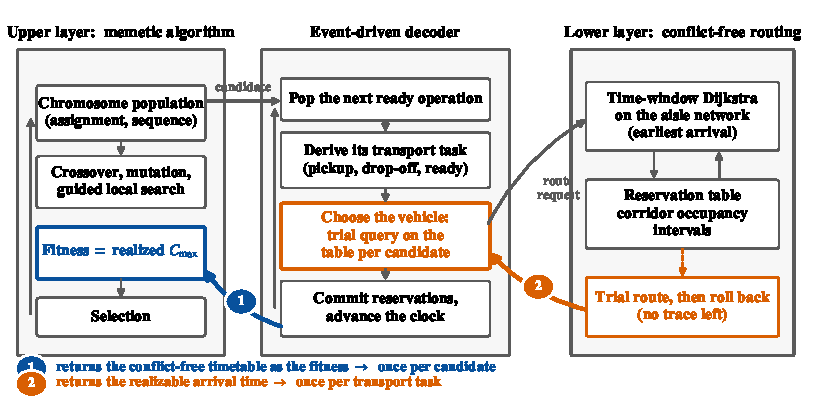
\includegraphics[width=0.8\textwidth]{fig/fig_framework.pdf}
\caption{The closed-loop bilevel framework.
Blue path~1 returns the conflict-free timetable as fitness, once per candidate.
Orange path~2 runs a two-leg trial query for the earliest feasible delivery before a vehicle is chosen; the trial query does not write the final timetable.
The ladder of Section~\ref{sec:Chapter_V} is arranged by whether these two paths are open.}
\Description{Schematic of the closed-loop bilevel framework: an upper memetic
search layer, an event-driven decoder, and a lower time-window reservation
routing layer, with two colour-coded feedback paths entering the upper layer at
different places---the evaluation path returning a realized makespan once per
candidate, and the decision path returning a realizable arrival time once per
transport task.}
\label{fig:framework}
\end{figure*}

\subsection{Lower level: time-window reservation and conflict-free routing}
\label{sec:router}

The only contended resource is the corridor (A6).
The reservation table maps each corridor to a time-ordered list of half-open occupancies $[t,\,t+\tau_e)$, labelled by vehicle and task, and supports four operations: earliest feasible entry no earlier than a given instant; write; revoke a task; and checkpoint/rollback for a trial query.
Nodes are not reserved: traversal takes zero time, waits occur at berths (A6).
The router and an independent checker inspect only corridor occupancy.

A leg is planned by a label-setting search (Algorithm~\ref{alg:route}).
A label $(u,t)$ means standing at the berth of $u$ at time $t$; the cost is $t$.
Querying the table for the earliest entry $t'\ge t$ produces the wait $t'-t$ of \eqref{eq:walk} directly.
Within one decode, written paths are not revoked, so vehicles are planned in decoder order and a later vehicle yields to an earlier one.

\begin{lem}[Earliest arrival is sufficient]
\label{lem:label}
Keeping only the earliest-arrival label at each node is sufficient to obtain a path that reaches the destination earliest under the current reservation table.
\end{lem}

\begin{proof}
  Berths have ample capacity and do not occupy the traversal resource (A6), so a vehicle that has stood at $u$ since time $t$ need only wait further until $t'$
  in order to take any continuation that a vehicle arriving at $u$ only at $t'>t$ could take.
  An earlier-arrival label is therefore never worse, and each node need keep only the earliest arrival.
  Moreover, the later the query time to the reservation table, the fewer the still-feasible entry slots,
  so the time to enter corridor $e$ and finish traversing it,
  $t\mapsto R.\textsc{EarliestEntry}(e,t,\tau_e)+\tau_e$,
  is non-decreasing in $t$.
  The search extracts labels in increasing order of arrival time; the first time the destination is extracted is the earliest arrival.
\end{proof}

Ordinary Dijkstra therefore suffices; there is no need for the per-interval labelling of Safe Interval Path Planning (SIPP)~\cite{kasaura2022sipp}.
A second criterion (a surcharge on busy slots) would force a multi-label Pareto search; Section~\ref{sec:interface} returns to that cost.

\begin{algorithm}[t]
  \caption{\textsc{Route}: conflict-free planning of a single leg}
  \label{alg:route}
  \footnotesize
  \begin{algorithmic}[1]
  \Require origin $s$, destination $g$, earliest departure $t_0$, table $R$, commit flag
  \Ensure occupancy intervals; written to $R$ if commit
  \State push $(s,t_0)$ onto a priority queue keyed by (time, node id)
  \While{the queue is nonempty}
    \State extract the least-key label $(u,t)$
    \If{$u=g$}
      \State backtrack occupancies; if commit, write them to $R$; \Return $t$
    \EndIf
    \ForAll{corridors $e=(u,v)$ leaving $u$}
      \State $t_{\text{in}} \gets R.\textsc{EarliestEntry}(e,t,\tau_e)$
      \State if $t_{\text{in}}+\tau_e$ is strictly earlier than the incumbent at $v$, update $(v,\,t_{\text{in}}+\tau_e)$
    \EndFor
  \EndWhile
  \State \Return failure \Comment{$G$ strongly connected: see text}
  \end{algorithmic}
\end{algorithm}

A path always exists: reservations are finite, time is bounded, and $G$ is strongly connected, so in the worst case the vehicle waits until every occupancy has ended and then takes an unimpeded shortest path.
That is the existence half of Proposition~\ref{prop:decodable}.
A single call costs $O\bigl(|E|\,(W^{2}+\log|V|)\bigr)$: at most $|E|$ corridors are examined; for each, $O(W)$ candidate entries are tested for overlap in $O(W)$ time, plus a heap step of $O(\log|V|)$, where $W$ is the mean number of reserved intervals per corridor.
A logarithmic earliest-entry query would drop this to $O\bigl(|E|(\log W+\log|V|)\bigr)$; this paper uses the linear scan.

The same search on an empty table over all pickup--delivery pairs yields the unimpeded matrix $t^{*}$ of Section~\ref{sec:Chapter_III}, used for open-loop arrival estimates, the reassignment neighbourhood, the two-stage baseline, and the admissible bound of Section~\ref{sec:speedup}.


\subsection{Upper level: encoding and event-driven decoding}
\label{sec:upper}

Let $N$ be the number of operations.
An individual has two segments: a machine-assignment vector of length $N$, the $k$-th entry an arm from $\Omega_{ji}$; and an operation sequence in which job $j$ appears $n_j$ times, the $x$-th appearance standing for $O_{jx}$.
The relative order of operations that share an arm is read from the sequence.
When $\delta_{\mathrm{ret}}=1$, each job appears once more for the dummy of Section~\ref{sec:Chapter_III}, so return transport needs no extra decoder branch.
Vehicle assignment is decided at decode time (Section~\ref{sec:dispatch}): a third segment would enlarge the search space and would no longer guarantee that every chromosome is decodable.

The decoder (Algorithm~\ref{alg:decode}) \emph{is} the evaluation path.
It sweeps the operation sequence from left to right, maintaining the idle time of each robotic arm, the current node and ready time of each job, and the current node and available time of each vehicle.
When the arm of an operation differs from the job's current location, a transport task of \eqref{eq:tasks} is generated, a vehicle is chosen, and two paths are planned against the \emph{live} reservation table: an empty leg to the pickup and a loaded leg to the destination, joined by \eqref{eq:load}.
The operation then starts by \eqref{eq:bind}; the decoder also records which of the two arguments is larger, as a \texttt{bind} field, which later attribution of a postponed start takes as authoritative.

\begin{algorithm}[t]
\caption{\textsc{Decode}: fitness from a complete conflict-free simulation}
\label{alg:decode}
\footnotesize
\begin{algorithmic}[1]
\Require instance, assignment $x$, operation sequence
\Ensure makespan, timetable, per-corridor yield statistics
\State $F_m\gets 0$ for every arm; $\mathrm{pos}_j\gets v_0$, $\mathrm{ready}_j\gets 0$ for every job
\State $\mathrm{loc}_k\gets v_0$, $\mathrm{avail}_k\gets 0$ for every vehicle; clear $R$
\ForAll{operations $O_{ji}$ in sequence order (dummies included)}
  \State $m\gets$ arm of $O_{ji}$ under $x$; $d\gets \mathrm{loc}(m)$
  \If{$\mathrm{pos}_j=d$}
     \State $A_{ji}\gets \mathrm{ready}_j$
  \Else
     \State choose vehicle $k$ (Section~\ref{sec:dispatch})
     \State $a^{\mathrm{E}}\gets\textsc{Route}(\mathrm{loc}_k,\mathrm{pos}_j,\mathrm{avail}_k,R,\text{true})$
     \State $\ell\gets\max(a^{\mathrm{E}},\mathrm{ready}_j)$
     \State $A_{ji}\gets\textsc{Route}(\mathrm{pos}_j,d,\ell,R,\text{true})$; $\mathrm{loc}_k\gets d$; $\mathrm{avail}_k\gets A_{ji}$
     \State accumulate yielding wait by corridor
  \EndIf
  \State $\texttt{bind}\gets\texttt{machine}$ if $F_m>A_{ji}$, else $\texttt{arrive}$
  \State $S_{ji}\gets\max(A_{ji},F_m)$; $C_{ji}\gets S_{ji}+p_{ji}$; $F_m\gets C_{ji}$; $\mathrm{pos}_j\gets d$; $\mathrm{ready}_j\gets C_{ji}$
\EndFor
\State \Return $C_{\max}=\max_{j,i} C_{ji}$, the timetable, and the yield statistics
\end{algorithmic}
\end{algorithm}

Reservations are written in decoder order; ties break by a fixed rule at both sites---the routing queue is keyed by (arrival time, node id) and updates only on a strictly earlier arrival; dispatching scans vehicles by increasing id and keeps the first strictly better one (Section~\ref{sec:speedup}).
A chromosome therefore maps to a unique timetable, so the seed-paired comparisons of Section~\ref{sec:Chapter_V} are deterministic.

\begin{prop}[Every chromosome is decodable]
  \label{prop:decodable}
  For any machine assignment and any operation sequence, Algorithm~\ref{alg:decode} terminates and returns a conflict-free, deadlock-free timetable of finite makespan. The search therefore need not invoke a repair operator.
\end{prop}

\begin{proof}
  By the encoding, the operation sequence is a topological order of each job's precedence constraints: the $x$-th appearance of a job stands for its $x$-th operation, so $\mathrm{ready}_j$ is already known when it is read.
  Ample buffers (A4) mean that an operation is never blocked for lack of storage, so once the job has arrived, \eqref{eq:bind} always supplies a finite start time.
  Each \textsc{Route} call returns in finite time by the argument after Algorithm~\ref{alg:route}, and occupies only a still-free slot on the reservation table, so \eqref{eq:excl} holds by construction.
  Deadlock-freedom is likewise by construction: the corridor is the only contended resource (A6); waits occur only at ample berths and do not occupy corridors; every occupancy written to the table ends at a finite time, so there is no mutually waiting fleet---in the worst case a vehicle waits until every existing occupancy has ended and then proceeds.
  The sweep executes $N+n\delta_{\mathrm{ret}}$ times, and each time schedules a finite number of events at finite times.
\end{proof}

The outer search is a conventional genetic algorithm, so the gains of Section~\ref{sec:Chapter_V} can be attributed to the mechanisms above rather than to operator tuning.
The initial population is random (uniform arm from $\Omega_{ji}$, shuffled sequence), plus two seeds: every operation on its fastest arm, and a load-balance greedy.
Selection is tournament with a small elite; the sequence uses precedence-preserving order crossover, the assignment uniform crossover; mutation swaps two sequence positions or moves an operation to another optional arm.
Fitness is the decoded makespan; hyperparameters are in Section~\ref{sec:impl}.

\subsection{Reservation-table-aware dispatching}
\label{sec:dispatch}

A vehicle may be chosen either by an unimpeded-shortest-path estimate or by a trial query on the reservation table.
The open-loop rule scores each vehicle by
\begin{equation}
\label{eq:rule}
\mathrm{score}(k)=\max\bigl(\mathrm{avail}_k+t^{*}(\mathrm{loc}_k,\text{pickup}),\,
\mathrm{ready}_j\bigr)+t^{*}(\text{pickup},\text{destination}),
\end{equation}
which does not consult the reservation table and may therefore select a vehicle that is geometrically near but whose corridor is already occupied.
The formula is the same as the idle-first dispatching of~\cite{li2026framework}, and is a typical single-attribute rule in surveys of multi-AGV dispatching~\cite{lu2022agv}.

The closed-loop default is instead \emph{reservation-table-aware dispatching}.
For each candidate vehicle, the empty leg is planned and temporarily written to the reservation table, the loaded leg is then planned against that state, the earliest feasible delivery time is recorded, and the table is rolled back to its state before the trial query.
The empty leg must be written temporarily; otherwise the loaded leg cannot see its occupancy, the two legs may be placed in the same corridor--time slot, and the trial query would be optimistically early.
The vehicle with the earliest feasible delivery is selected, not the vehicle that \eqref{eq:rule} estimates as best.

Vehicles have identical capability (assumption~A5) and differ only in current location and corridor occupancy, so contention on the reservation table determines the choice.

The trial query raises routing calls per transport from $2$ to at most $2N_A$, about \CostMultBefore{} times an unimpeded-time selection.
Without the speed-ups of Section~\ref{sec:speedup}, this overhead offsets the makespan gain under an equal wall-clock budget; Section~\ref{sec:Chapter_V} therefore compares the two rules only under the same wall-clock limit.

\subsubsection{Three choices for the inter-layer interface}
\label{sec:interface}

With the two levels fixed, the remaining choice is what the lower level returns.
This paper implements three interfaces and measures each under an equal wall-clock budget; only the first reduces makespan (Section~\ref{sec:Chapter_V}).

\paragraph{Return realized durations only.}
The lower level returns traversal times after conflict-free routing---the evaluation path, and the quantity that a trial query reads.
Every candidate is ranked by the makespan after yielding wait; schedule-then-route methods see that duration only after the assignment is fixed.

\paragraph{Return a surcharge on corridor--time slots.}
A shadow price $\pi(e,b)$ is attached to each occupied corridor--time slot; path planning then minimizes ``arrival time $+\theta\cdot$cost'' on the Pareto front ($\theta\ge0$ is the only knob).
Two estimates are implemented: perturbing one slot and re-solving, and a low-cost approximation refreshed each generation.
Contention wait already enters arrival time and, through \eqref{eq:bind}, makespan, so the surcharge adds no new information.
It also adds cost: by Lemma~\ref{lem:label}, price is a second criterion, so single-label Dijkstra must become a multi-label Pareto search whether or not a surcharge is finally applied.
Under an equal wall-clock budget makespan consistently worsens, and Section~\ref{sec:Chapter_V} attributes the loss mainly to this search overhead.

\paragraph{Return the yield record.}
A yield triple (corridor, time slot, preceding transport) generates the local-search neighbourhood of Section~\ref{sec:ls} without double-counting the delay.
Under an equal wall-clock budget the neighbourhood is well targeted, but its hit rate does not offset the extra evaluations.

\subsection{Low overhead: admissible lower-bound pruning and winner-path reuse}
\label{sec:speedup}

At equal generation count the trial query beats rule-based dispatching by \GainProbeSameGen{}, but one evaluation is \CostMultBefore{} times more expensive, so under equal wall-clock time the gain is offset and the net effect is almost zero.
The two optimizations below lower the evaluation cost without changing any selection.

\paragraph{Admissible lower-bound pruning.}
Conflict-free routing can only become later because of yielding; it can never be faster than the unimpeded shortest path.
The open-loop score \eqref{eq:rule} is therefore an \emph{admissible lower bound} on the realized delivery time:
\begin{equation}
\label{eq:lb_dispatch}
\mathrm{lb}(k)=\max\bigl(\mathrm{avail}_k+t^{*}(\mathrm{loc}_k,\text{pickup}),\,
\mathrm{ready}_j\bigr)+t^{*}(\text{pickup},\text{destination})\ \le\ \mathrm{est}(k),
\end{equation}
where $\mathrm{est}(k)$ is the earliest feasible delivery time obtained by a complete two-leg trial query for vehicle $k$.
Hence if a vehicle's lower bound is already no earlier than the current best trial-query delivery, routing need not be called for it.

\paragraph{Winner-path reuse.}
After the trial query the reservation table is rolled back as a whole, the winner's two legs included; the decoder then recomputes them, wasting two routing calls.
What $\textsc{Route}(\cdot,\textit{commit}=\text{true})$ does is merely write the legs into the reservation table in order, so the paths already computed for the winner during the trial query can be cached and committed directly, without replanning.

\begin{prop}[The two speed-ups do not change the selected vehicle or the timetable]
  \label{prop:speedup_equiv}
  In the implementation, vehicles are queried in increasing id order, and the selected vehicle is replaced only when some vehicle's feasible delivery is strictly earlier than the current best.
  Under this rule, after the pruning of \eqref{eq:lb_dispatch} and winner-path reuse are added, the selected vehicle, the occupancies written to the reservation table, and the final timetable are the same as when a complete two-leg trial query is run for every vehicle.
\end{prop}

\begin{proof}
  Consider pruning first.
  When vehicle $k$ is reached, let the current best trial-query delivery be $\mathrm{est}^{\ast}$.
  If $\mathrm{lb}(k)\ge \mathrm{est}^{\ast}$, then \eqref{eq:lb_dispatch} gives
  $\mathrm{est}(k)\ge\mathrm{lb}(k)\ge\mathrm{est}^{\ast}$,
  so $k$'s feasible delivery cannot be strictly earlier and would not be selected even if every vehicle received a complete trial query; not calling routing for it leaves the selected vehicle unchanged.
  The reservation table is saved before each trial query and restored afterwards; vehicles for which routing is not called do not rewrite the table and therefore do not affect later queries.
  Consider reuse next: the two legs of the selected vehicle were computed against the same reservation-table state; after restore, the table is the same state the decoder later writes into.
  $\textsc{Route}(\cdot,\textit{commit}=\text{true})$ only writes the given legs into the table, so writing the cached paths and replanning then writing produce identical occupancy intervals.
\end{proof}

Together the two optimizations give a \SpeedupProbe{}-fold speed-up, cut routing calls by \RouteCallCut{}, and reduce the cost multiple of a single evaluation from \CostMultBefore{} to \CostMultAfter{}.
These three numbers are the \emph{joint} effect of the two: the experiment measures them as one on/off switch (Table~\ref{tab:prune}), and this paper does not attribute them separately to pruning or reuse.

The effect of pruning varies with fleet size.
The tighter the bound and the earlier a good trial-query delivery is obtained, the more vehicles need not call routing; the larger the fleet, the more candidates, and the total trial-query cost grows approximately linearly with $N_A$.
Section~\ref{sec:Chapter_V} reports the measurement: the pruning effect weakens as the fleet grows, but still cuts \RouteCallCutLo{} of the routing calls on the largest fleet tested.
The two effects together mean that the gain of the mechanism may vanish after the fleet reaches some size; Section~\ref{sec:whichcongestion} explains why the present number of seeds is not sufficient to identify that size.

\subsection{Yield-record-guided local search}
\label{sec:ls}

The third interface of Section~\ref{sec:interface} is written as local-search operators on a typed critical chain (Table~\ref{tab:attrib}).
Backtracking from the event that attains the makespan includes transport legs as well as operations, and labels each link as \texttt{operation}, \texttt{machine}, \texttt{upstream}, \texttt{vehicle}, or \texttt{corridor}.
A yield on a loaded leg is always \texttt{corridor}; on an empty leg, a yielding share above $0.5$ distinguishes \texttt{corridor} from \texttt{vehicle}.
The same labels are used to read the case study of Section~\ref{sec:casestudy}.

\begin{table}[t]
  \caption{Critical-chain labels.
  Only \texttt{corridor} names a concrete corridor, time slot, and occupying transport.}
\label{tab:attrib}
\footnotesize
\begin{tabular}{@{}llp{2.55cm}@{}}
\toprule
Label & Criterion & Remedy \\
\midrule
\texttt{operation} & a real operation is occupying its robotic arm & --- \\
\texttt{machine} & $\texttt{bind}=\texttt{machine}$, blocked by the preceding operation on that arm
  & resequence \\
\texttt{upstream} & the vehicle arrived first, the material is not yet ready & recurse to $O_{j,i-1}$ \\
\texttt{vehicle} & the material is ready, the vehicle is late, and yielding is a small share of the delay & change vehicle \\
\texttt{corridor} & a yield occurs on a specified corridor at a specified time slot & reassignment or staggering \\
\bottomrule
\end{tabular}
\end{table}

Two operators use the yield record.
Reassignment scores each alternative arm $m'\in\Omega_{ji}\setminus\{m\}$ of at most $L=5$ real operations on the chain by
\begin{equation}
\label{eq:reassign}
\mathrm{score}(m')=t^{*}\bigl(\mathrm{pos}_{j,i-1},\mathrm{loc}(m')\bigr)
+t^{P}_{jim'},
\end{equation}
unimpeded travel plus processing time; the lowest-scoring arm produces a neighbour that changes only that assignment, which is the trade-off of this paper (a nearer arm may be slower).
Staggering takes the longest \texttt{corridor} link and either advances the blocked operation or postpones the occupier; each round moves one operation, so the result remains a legal permutation and, by Proposition~\ref{prop:decodable}, remains decodable.
The neighbourhood has at most $L+2=7$ candidates.
Each selected individual is given at most three first-improvement rounds, and the chain is recomputed after every acceptance.
Under an equal wall-clock budget this interface does not yield a stable makespan gain (Section~\ref{sec:Chapter_V}).

\subsection{Complexity and cost}
\label{sec:complexity}

One fitness evaluation processes $N+n\delta_{\mathrm{ret}}$ events.
Under closed-loop dispatching each transport uses at most $2N_A$ routing calls, so each individual costs
$O\bigl((N+n)\,N_A\,|E|\,(W^{2}+\log|V|)\bigr)$; open-loop selection by unimpeded time no longer carries the factor $N_A$.
The lower-bound pruning of Section~\ref{sec:speedup} does not change this worst-case bound, but by Proposition~\ref{prop:speedup_equiv} it reduces the actual number of calls by \RouteCallCut{} without changing the output, i.e.\ it replaces $N_A$ by a smaller effective multiple.
Local search adds at most $3(L+2)$ further evaluations for each selected individual.

Within the framework, the cost of a single evaluation can differ by about two orders of magnitude.
On the ladder batch the measurements are: open-loop \MsOpen{}\,ms, closed-loop rule-based dispatching \MsLoopRule{}\,ms, full closed-loop \MsLoopProbe{}\,ms, about $37$ times the open loop.
Pricing is not in that batch; it comes from an earlier pricing scan; within that batch, turning pricing on raises a single evaluation from \MsPricedRef{}\,ms to \MsPriced{}\,ms, another factor of about $4.8$.
The absolute milliseconds of the two batches must not be divided into each other; the product of the two multiples already shows the span: the most and least expensive configurations differ by about two orders of magnitude in the cost of a single evaluation.
Equal generation counts are therefore not an appropriate comparison, and Section~\ref{sec:Chapter_V} aligns wall-clock time instead.

This framework does not prove convergence to a fixed point.
The lower level plans sequentially, not jointly to optimality; the upper level is a randomized search on a non-convex space; what crosses the interface is a duration or a yield record, not a Lyapunov function.
Proposition~\ref{prop:decodable}, Lemma~\ref{lem:label}, and Proposition~\ref{prop:speedup_equiv} give a narrower guarantee that is enough for a heuristic: every candidate is feasible, its evaluation matches the conflict model of Section~\ref{sec:Chapter_III}, and the two speed-ups do not change any selection; together with the deterministic decode of Section~\ref{sec:upper}, the process is reproducible.
Solution quality is given by the experimental protocol of the next section.

